\chapter{数据库通信协议分析}
本章主要通过使用 Wireshark 对各种数据库的协议进行分析,以便在 Suricata 中加入协议分析代码,实现最终的 IDS/IPS 功能。其中涉及的协议有 MySQL、DB2、SQL Server 以及 Oracle。由于 Wireshark 已经完整支持了前三者的通信协议,本章着重分析 Oracle 的 TNS 协议。

\begin{quote}
为便于后续维护,以避免不同 Wireshark 版本带来的差异,现列出本版本的 Wireshark 帮助信息。

\begin{figure}[h!]
    \centering
    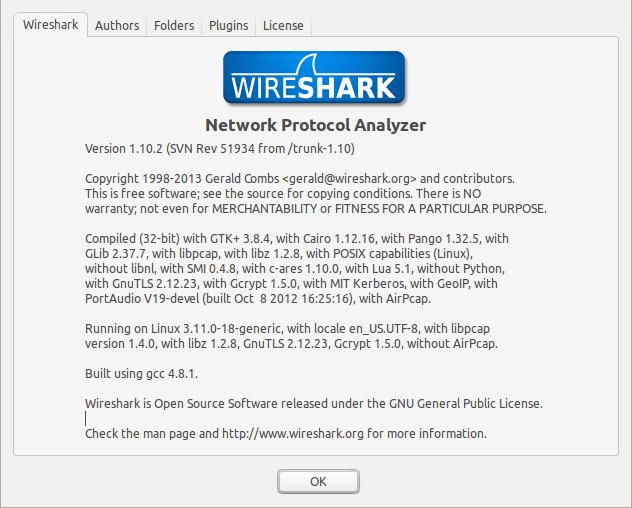
\includegraphics[width=0.8\textwidth]{wireshark.png}
\end{figure}
\end{quote}

\section{Oracle 数据包协议分析}
由于 Wireshark 对 Oracle 数据包的支持不够,所以需要做一些反向工作,将 Oracle 中的 TNS 协议以及 Net8 协议分析出来。\footnote{关于 Oracle 数据库的通信模型,\href{http://docs.oracle.com/cd/A57673\_01/DOC/net/doc/NWUS233/ch2.htm}{这里}有一个它的 SQL*Net 文档。}。

\begin{quote}
    本文 Oracle 客户端使用的 sqlplus 版本为 {\ef SQL*Plus: Release 12.1.0.1.0 Production},服务器端的版本为 {\ef Oracle 11g R2}。其它版本的分析结果可能会有所差异,需后续跟进。
\end{quote}

Oracle 数据库操作也分为三个步骤,首先需要登陆,这期间客户端和服务器端交换一些通信数据,比如版本、用户认证、Session 注册等等。登陆成功后,才能对数据库中的数据进行操作。操作完成后,再退出登陆。完成一次数据库交互。

Oracle 使用的 TNS 协议是私有协议,官方并未将协议的 Spec 放出来。但是各路大侠们捕风捉影,也能拿到一些靠谱的信息。对一个 TNS 数据包而言,它由两部分组成,一部分是头部数据,长度为 8 个字节(如果加上载荷上前面无用的 2 个字节,就是 10 个字节),其中包括长度、类型等信息。另一部分为载荷数据,其中包含了具体的数据包内容。本节主要分析其载荷数据。因为头部数据在 Wireshark 中已经可以完整查看。

关于头部的数据包类型字段,现收集如表 \ref{tab:oracle-tns-data-type} 所示,以供参考。

\begin{table}[!h]
    \centering
    \caption{Oracle TNS 协议中数据类型列表}
    \begin{tabular}{|>{\cf\scriptsize}r|>{\scriptsize}l|>{\cf\scriptsize}r|>{\scriptsize}l|>{\cf\scriptsize}r|>{\scriptsize}l|} \hline
        字节  & 意义              & 字节 & 意义           & 字节 & 意义                   \\ \hline\hline
         0x01 & Connect           & 0x06 & Data           & 0x11 & Resend                 \\ \hline
         0x02 & Accept            & 0x07 & NULL           & 0x12 & Marker                 \\ \hline 
         0x03 & ACK               & 0x08 & ---            & 0x13 & Attention              \\ \hline
         0x04 & Refuse            & 0x09 & Abort          & 0x14 & Control                \\ \hline
         0x05 & Redirect          & 0x10 & ---            &      &                        \\ \hline
    \end{tabular}
    \label{tab:oracle-tns-data-type}
\end{table}

对 TNS 协议中的载荷数据而言,它也有不同的类型,该类型字段位于载荷数据包的前面两个字节(即应用层数据包偏移 10 个字节),其类型如表 \ref{tab:tns-payload-data-type} 所示:

\begin{table}[!h]
    \centering
    \caption{Oracle TNS 协议中载荷数据包类型}
    \begin{tabular}{|>{\cf}r|>{\scriptsize}p{6cm}|} \hline
        字节  & 意义               \\ \hline\hline
         0x01 & Protocol Negotiation. Following this flag are acceptable protocol versions {\cf\scriptsize 0x060504030201} and client platform string like {\cf\scriptsize IBMPC/WIN\_NT-8.1.0} \\ \hline
         0x02 & Exchange of Data type representations. \\ \hline 
         0x03 & TTI (Two-Task Interface) Function call. The exact function id comes immediately after data packet id. \\ \hline 
         0x08 & ``OK'' server to client response \\ \hline
         0x11 & Extended TTI (Two-Task Interface) Function call. \\ \hline
         0x20 & Used by external procedures and service registrations \\ \hline
         0x44 & Used by external procedures and service registrations \\ \hline
         0xdeadbeef & Additional Network Options. Client may negotiate additional connection attributes such as authentication, encryption, data integrity, and supervisor.\\ \hline
    \end{tabular}
    \label{tab:tns-payload-data-type}
\end{table}

其中对{\cf 0x11} 类型的数据而言,其后面会紧跟以下几种类型的数据:

\begin{itemize}
    \item {\cf 0x6b}: switch to detach session
    \item {\cf 0x78}: close
    \item {\cf 0x87}: OSCID
    \item {\cf 0x9a}: OKEYVAL
\end{itemize}

对 {\cf 0x03} 类型的载荷而言,其后面所紧跟的种类在表 \ref{tab:oracle-tns-tti} 中列出。

\subsection{Oracle 登陆数据包的组成}
对登陆而言,其来往的数据包多达几十条,除了登陆数据包之外(类型为 {\cf 0x01}),客户端发往服务器端的数据包(类型为 {\cf 0x06})还有如下几种,其中的字节列举的是 payload 中的首部字节。

\begin{enumerate}
    \item 客户端发往服务器端的标有 ``网络连接属性'' 的数据包({\cf 0xdeadbeef})
    \item 协议数据包,客户端需要更服务器端对接数据通信协议({\cf 0x01})
    \item 交换 ``数据表示形式'' 的数据包 ({\cf 0x02})
    \item 带用户名和密码的两个登陆数据包,此处的用户名和密码放在两个数据包中传送({\cf 0x0376, 0x0373})
    \item 确定服务器数据库信息的数据包({\cf 0x116b})
    \item 一个带有 SQL 语句的数据包,其中的 SQL 语句为 {\cf SELECT USER FROM DUAL},该数据包会返回用户当前的登陆用户名({\cf 0x035e}) 
    \item 一个 Fetch 数据包({\cf 0x0305}) 
    \item ({\cf 0x1169}) 发送一个 SQL 语句 {\cf BEGIN DBMS\_OUPUT.DISABLE; END;}
    \item ({\cf 0x1169}) 发送一个 SQL 语句 {\cf BEGIN DBMS\_APPLICATION\_INFO.SET\_MODULE(:1, NULL); END;}
    \item ({\cf 0x1169}) 发送一个 SQL 语句 {\cf SELECT DECODE('A', 'A', '1', '2') FROM DUAL;}
    \item ({\cf 0x030e}) 发送一个 COMMIT 请求,完成登陆过程。
\end{enumerate}

对服务器端而言,其返回的 payload 数据包中如果以 {\cf 0x08} 开头,则证明请求通过。对首部为 {\cf 0x03} 的登陆数据包而言(即 TTI,{\ef two-task interface}),其后面跟着的字节分别表示各种意义,如表 \ref{tab:oracle-tns-tti} 所示:

\begin{table}[!h]
    \centering
    \caption{登陆数据包中以 {\cf 0x03} 为首字节的 TTI 字节列表}
    \begin{tabular}{|>{\cf}r|>{\scriptsize}r|>{\cf}r|>{\scriptsize}r|>{\cf}r|>{\scriptsize}r|} \hline
        字节  & 意义              & 字节 & 意义           & 字节 & 意义             \\ \hline\hline
         0x02 & Open              & 0x0f & Rollback       & 0x5c & OKOD             \\ \hline
         0x03 & ---               & 0x14 & Cancel         & 0x5e & Query            \\ \hline 
         0x04 & Execute           & 0x2b & Describe       & 0x60 & LOB Operations   \\ \hline
         0x05 & Fetch             & 0x30 & Startup        & 0x62 & ODNY             \\ \hline
         0x08 & Close             & 0x31 & Shutdown       & 0x67 & Transaction-end  \\ \hline
         0x09 & Disconnect/logoff & 0x3b & Version        & 0x68 & Transaction-begin\\ \hline
         0x0c & AutoCommit On     & 0x43 & K2 Transactions& 0x69 & OCCA             \\ \hline
         0x0d & AutoCommit Off    & 0x47 & Query          & 0x6d & Startup          \\ \hline
         0x0e & Commit            & 0x4a & OSQL7          & 0x51 & Logon            \\ \hline
         0x52 & Logon             & 0x73 & Logon          & 0x76 & Logon            \\ \hline
         0x77 & Describe          & 0x7f & OOTCM          & 0x8B & OKPFC            \\ \hline
    \end{tabular}
    \label{tab:oracle-tns-tti}
\end{table}

\begin{quote}
    表 \ref{tab:oracle-tns-tti} 中出现了多个重复意义的字段,它们各自的实际意义如下:

    \begin{itemize}
        \item {\cf 0x5e}:指一般的 SQL 语句查询
        \item {\cf 0x47}:在现有的分析中没有碰到这种类型的查询字段
        \item {\cf 0x30} 和 {\cf 0x60} 虽然都为 Startup,但是尚未碰到这种数据包
        \item {\cf 0x51}:带密码的登陆行为
        \item {\cf 0x52}:带用户名的登陆行为
        \item {\cf 0x73}:带密码的登陆行为,其中带有 {\cf AUTH\_PASSWORD} 信息
        \item {\cf 0x76}:带用户名的登陆行为,其中带有 {\cf AUTH\_SESSKEY} 信息
    \end{itemize}
\end{quote}

由于登录数据包中类型为 {\cf 0x01}、{\cf 0x011} 以及 {\cf 0x02} 数据包在 Wireshark 中能正确识别,所以就不做详细分析,只列出其基本的组成。对 {\cf 0x01} 类型的数据包而言,它是客户端发给服务器端的第一个连接数据包,其字节组成如下

\begin{lstlisting}
    TNS connect pkt
    |
    +- [2B] pkt len
    +- [2B] pkt checksum 一般为 0x0000
    +- [1B] pkt type
    +- [1B] reserved byte
    +- [2B] header checksum
    +- [2B] version
    +- [2B] compitible version
    +- [2B] service option,其中有各种 bit 位,详见 Wireshark 结果
    +- [2B] session data unit size
    +- [2B] maximum transimission data unit size
    +- [2B] NT protocol characteristics,各种 bit 位参见 Wireshark 结果
    +- [1B] line turnaround value
    +- [2B] value of 1 in hardware
    +- [2B] length of connect data
    +- [2B] offset to connect data
    +- [4B] maximum receivable connect data
    +- [1B] connection flags,各种 bit 位参见 Wireshark 结果
    +- [...]
    +- [nB] connect data
\end{lstlisting}

对于用 sqlplus 登陆的客户端而言,当客户端第一次发送连接数据包之后,服务器端往往会要求客户端重传({\cf 0x11})这次连接数据包。\footnote{重传的目的尚不明确。在老版本 Oracle 的协议中(Oracle 9i),Server 端会将客户端定位到另一个端口进行通信,而不是默认的 1521。在最近的版本中,已经移除了这个设定。}
重传的数据包中,应用层的数据包与前一次的字节全部相同。服务器端验证通过后,会发送 Accept 数据包({\cf 0x02}),其数据包结构为

\begin{lstlisting}
    TNS accept pkt
    |
    +- [2B] pkt len
    +- [2B] pkt checksum 一般为 0x0000
    +- [1B] pkt type
    +- [1B] reserved byte
    +- [2B] header checksum
    +- [2B] version,此 version 值可能会低于客户端传送过来的 version值
    +- [2B] service option,其中有各种 bit 位,详见 Wireshark 结果
    +- [2B] session data unit size
    +- [2B] maximum transimission data unit size
    +- [2B] value of 1 in hardware
    +- [2B] accept data length
    +- [2B] offset to accept data
    +- [2B] connect flag,在 Wireshark 中看来是两个相同的字节,意义不大
\end{lstlisting}

接下来,在 Wireshark 中会看到两个 SNS 数据包,它们之间交换一些数据之后就进入正式的登陆流程。此处 SNS 数据包的类型也是 {\cf 0x06},其判断依据是检查 payload 上前面四个字节,如果为 {\cf 0xdeadbeef},则为 SNS 数据包。

\subsection{Oracle 查询数据包的组成}\label{sec:oracle-query-string}
从目前所观察的数据包来看,查询数据包是有一定规律的,如果只提取客户端的查询字符串,而不涉及 session 管理以及结果集的提取,那么这个过程是比较简单的。

首先,对于登陆后出现的第一个查询语句,其数据包结构是特殊的,其后续的查询数据包则以另外一种形态保持一致。下面以一系列 SQL 语句为例,来说明这个过程。

\lstinputlisting[language=sql,
numbers=left,
numberstyle=\tiny\color{gray},
numbersep=8pt,
caption={\ff h-query.sql},
stepnumber=1]{h-query.sql}

将这些 SQL 存为文件 {\ff h-query.sql}。登陆 Oracle 数据库库之后,在 sqlplus 控制台输入如下命令则执行该文件:

\begin{lstlisting}
SQL> @h-query.sql
\end{lstlisting}

在 Wireshark 中,第一个数据包如图 \ref{fig:tns-first-sql} 所示:

\begin{figure}[ht!]
    \caption{登陆后第一条 SQL 语句的数据包}
    \label{fig:tns-first-sql}
    \centering
    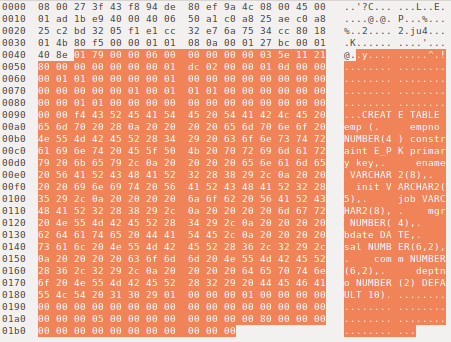
\includegraphics[width=0.9\textwidth]{tns-first-sql.png}
\end{figure}

橙色阴影下的数据即为应用层数据,除去前面的 10 个字节(头部 8 字节以及 2 字节的 data flag 字段),就是 {\cf CREATE TABLE} 命令的数据包载荷。

最先出现的字节是 {\cf 0x035e},从表 \ref{tab:oracle-tns-tti} 可以得知,字节 {\cf 0x5e} 代表一个 Query 操作,后面的 {\cf 0x11} 代表数据包序列号,这点可以从后续的 {\cf INSERT} 语句的载荷数据包中看出来,只是该序列号不是逐个递增的,而是间隔递增的,即后续的 Query 数据包的序列号为 {\cf 0x13}、{\cf 0x15}、{\cf 0x17}、$\cdots$。至于其原因,在后面提到时再说明。

再往后的字节尚不知道其具体含义。从序列号字段开始(payload + 3),跳过 67 个字节之后,到达 {\cf 0090} 这一行的第三个字节 {\cf 0x4f},它就是表示后面查询字符串的长度。该字节之后,就是具体的查询字符串,也即 {\cf CREATE TABLE} 语句。

\begin{quote}
    经测试,当 SQL 长度小于等于 {\cf 0xfc} 时(252),该字节就是后面数据包的长度。当 SQL 语句的长度超过 253 时,那么该字节固定为 {\cf 0xfe},后面紧跟的那个字节才是 SQL 的长度。此处 {\cf 0xfe} 是一个标记字符,它说明此时 SQL 语句的长度已经大于 {\cf 0xfc},例如当数据包长度为 {\cf 0xfd} 时,此时的数据包为

\begin{lstlisting}
+------+------+----------+
| 0xfe | 0xfd | sql stmt |
+------+------+----------+
\end{lstlisting}

当 SQL 的长度超过 {\cf 0xfe}(254)时,此时这两个字节都不能用来断定后续的 SQL 长度,因为此时这两个字节的长度固定为 {\cf 0xfeff},无法用它来断定后续的长度是 {\cf 0xff} 还是大于 {\cf 0xff}。此时,TNS 协议对数据包做了特殊处理,即如果 SQL 语句长度刚好 255 个字节,那就直接拷贝这 255 个字节,如果大于 255 字节,则每隔 255 个字节会在数据包中插入一个分隔字节(例如 {\cf 0x80},但该分隔字节不固定,会有变动),此时,通过总长度以及固定位置的分隔符,即可将被分割的 SQL 语句提取出来。

另一点值得注意的是,此处提到的 SQL 语句长度并不是输入 SQL 语句的长度,在 sqlplus 中会对 SQL 语句做预处理,目前看来至少去掉了其中不必要的空白字符。而且 sqlplus 会对 SQL 语句做基本的 SQL 解析,不合语法的 SQL 语句不会发送到服务器端。
\end{quote}

以上是登陆后第一条查询语句的数据包分析。接下来分析第一条查询之后的其他查询语句的数据包。这种数据包如图 \ref{fig:tns-successive-sql} 所示。

\begin{figure}[ht!]
    \caption{第一条 SQL 语句之后的数据包}
    \label{fig:tns-successive-sql}
    \centering
    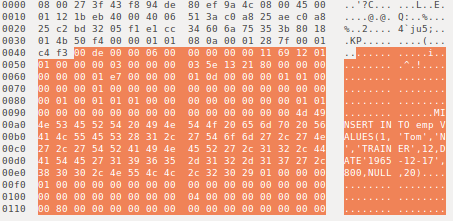
\includegraphics[width=0.9\textwidth]{tns-successive-sql.png}
\end{figure}

从图 \ref{fig:tns-successive-sql} 中可以看出,其载荷中的首部字节变成了 {\cf 0x1169},从表 \ref{tab:tns-payload-data-type} 可以得知,这是一个扩展的 TTI 数据包,其中 {\cf 0x69} 的意义为 {\ef Cursor Close All},此处对数据包的分析意义不大,但是后面紧跟着的是数据包的序列号 {\cf 0x12}。如何解释呢?此处的意义即这是一条独立计数的数据包。截止到字节 {\cf 0x035e} 为止,其长度为 12 字节。从 {\cf 0x035e} 开始,又开始了一条独立计数的数据包,其序列号为 {\cf 0x13},这就解释了上面 {\cf CREATE TABLE} 数据包中所提到的序列号间隔的问题。

在 {\cf 0x035e13} 之后,同样跳过 67 个字节,即可拿到后面 SQL 语句的长度字节 {\cf 0x4f},再之后就是具体的 {\cf INSERT} 语句。

至此,基本的客户端 SQL 语句的数据包分析完毕。接下来是一些其它信息的数据包分析。

注意到,在上面的批量 SQL 语句中,第二个 {\cf INSERT} 语句中的主键与第一条 {\cf INSERT} 语句是重复的,所以服务器端会报错,在我们的 Wireshark 中,肯定不会错过这一幕,对此,服务器会发送两种数据包,一种是 {\cf Attention} 数据包,一种是常规的类型为 {\cf 0x06} 的数据包,其中带有错误信息。这两个数据包分别如图 \ref{fig:tns-attention} 以及图 \ref{fig:tns-error-msg} 所示:

\begin{figure}[ht!]
    \caption{Oracle TNS 的 Attention 数据包}
    \label{fig:tns-attention}
    \centering
    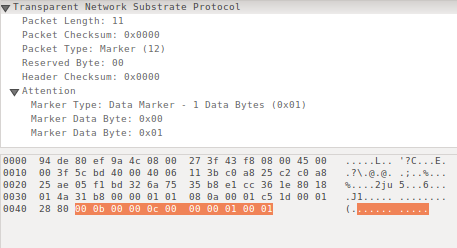
\includegraphics[width=0.9\textwidth]{tns-attention.png}
\end{figure}

因为 Attention 数据包中并无实质性的数据,它顶多只能算是一个暗示。后面的 Error Message 数据包才是有价值的。

\begin{figure}[ht!]
    \caption{Oracle TNS Error Message 数据包}
    \label{fig:tns-error-msg}
    \centering
    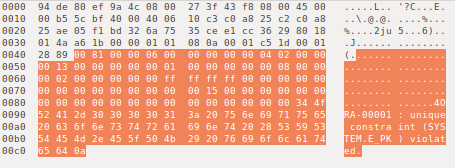
\includegraphics[width=0.9\textwidth]{tns-error-msg.png}
\end{figure}

此处载荷的头部字节为 {\cf 0x0402},可以确定是一个``错误信息'',其具体的错误描述则在 64 个字节之后。 {\cf 0080} 这一行的倒数第二个字节 {\cf 0x34},即为错误信息的长度,后面紧跟的就是具体的错误信息。从描述中,可以得知,此处违反了主键的唯一性约束。

接下来分析一下 {\cf SELECT} 语句的数据包,由于 {\cf SELECT} 语句有一个获取结果的过程,所以会出现一个 Fetch 数据包。在上面的批量 SQL 中,有一个 {\cf SELECT} 语句,其数据包和 {\cf INSERT} 语句没有实质性的差别,关键是其后面紧跟的 Fetch 操作。其数据包如图 \ref{fig:tns-fetch} 所示。

\begin{figure}[ht!]
    \caption{Oracle TNS Fetch 数据包}
    \label{fig:tns-fetch}
    \centering
    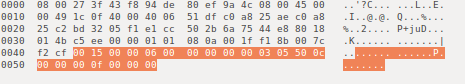
\includegraphics[width=0.9\textwidth]{tns-fetch.png}
\end{figure}

此处的载荷数据包头部字节为 {\cf 0x0305},从表 \ref{tab:oracle-tns-tti} 可以得知,这是一个 Fetch 操作,即 {\cf SELECT} 语句之后获取查询结果的操作。这个操作之后,服务器会返回 {\cf SELECT} 的结果,如图 \ref{fig:tns-select-result} 所示。

\begin{figure}[ht!]
    \caption{Oracle TNS SELECT 结果数据包}
    \label{fig:tns-select-result}
    \centering
    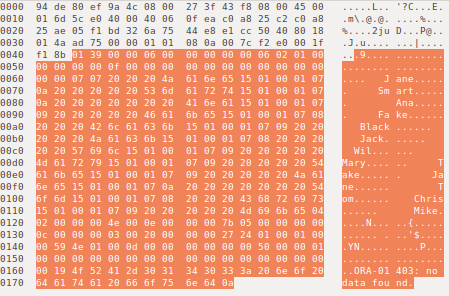
\includegraphics[width=0.9\textwidth]{tns-select-result.png}
\end{figure}

上面提到了一个数据包序列号的问题,目前来看,只有一个字节用来保存数据包的序列号,如果上面的 {\cf INSERT} 语句超过 256 个,那么这个序列号会回滚到 0 么?可以测试一下,写个 Python 脚本,生成这么堆 {\cf INSERT} 语句:

\lstinputlisting[language=python,
numbers=left,
numberstyle=\tiny\color{gray},
numbersep=8pt,
caption={\ff gen-long-insert.py},
stepnumber=1]{gen-long-insert.py}

用 sqlplus 将这几百个 {\cf INSERT} 语句喂给 Oracle 服务器之后,能拿到一大堆的数据包,其中,在第 214 条 {\cf INSERT} 语句中,其序列号达到了 {\cf 0xff}。
\footnote{因为前面的测试数据包已经``占用''了一部分序列号。}
其前后数据包如图 \ref{fig:tns-seq-rollback} 所示。

\begin{figure}[ht!]
    \caption{Oracle TNS 数据包序列号回滚现场}
    \label{fig:tns-seq-rollback}
    \centering
    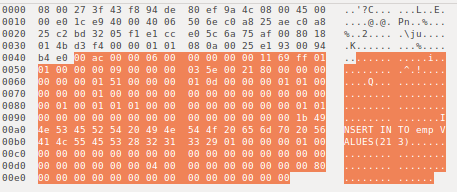
\includegraphics[width=0.9\textwidth]{tns-seq-rollback.png}
    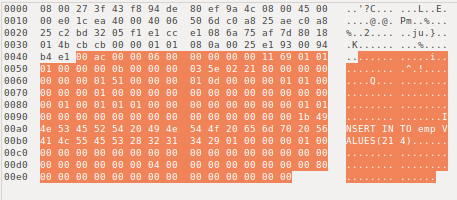
\includegraphics[width=0.9\textwidth]{tns-seq-rollback2.png}
\end{figure}

在第一个数据包中,{\cf 0x1169} 后面的序列号字节为 {\cf 0xff},到顶了,下一个 {\cf 0x035e} 的数据包序列号回滚到了 {\cf 0x00}。此即证明这种回滚的猜想是正确的,从其后面的那个数据包中,这一猜想也能得到印证。费了这么大劲搞序列号干什么用呢?

由于序列号的存在,使得客户端的请求必须按照``拿号''的顺序来,中间的插入者不能直接获取到这个序列号,有点类似于 TCP 中的 ACK,虽然此处服务器端并未将序列号传回给客户端,但是单边的序列号在一定程度上让服务器有一个验证依据。这期间发生的篡改也能被 IPS 所检测到。

\subsection{Oracle 中其它数据包分析}
为验证以上分析的严谨性,现收集一些其它数据包进行分析。

\lstinputlisting[language=sql,
numbers=left,
numberstyle=\tiny\color{gray},
numbersep=8pt,
caption={\ff update.sql},
stepnumber=1]{update.sql}

对于第一个 {\cf CREATE TABLE} 语句而言,其遵循前面的分析,载荷数据以 {\cf 0x1169} 开头,后面再跟进另一个数据包,以 {\cf 0x035e} 开头。对第 13 行的 {\cf SET} 语句而言,其在数据包中的字节并不是 SQL 语句,其数据包如图 \ref{fig:tns-set-output} 所示。

\begin{figure}[ht!]
    \caption{Oracle TNS 数据包与 SQL 语句不一致现场}
    \label{fig:tns-set-output}
    \centering
    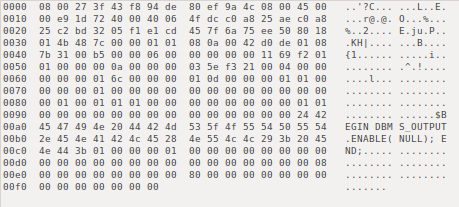
\includegraphics[width=0.9\textwidth]{tns-set-output.png}
\end{figure}

从数据包中的字节来看,实际传送给服务器的是这样一段 SQL 语句

\begin{lstlisting}[language=sql]
BEGIN DBMS_OUTPUT.ENABLE(NULL); END;
\end{lstlisting}

除此之外,字段偏移以及序列号,均遵循之前的分析。如果按照上文的做法,此处对 SQL 语句的记录可能会有偏差,虽然其结果可能是一样的。可以单独用这个 {\cf BEGIN} 语句测试一下其数据包的情况。

\begin{figure}[ht!]
    \caption{Oracle TNS 被转换后的 SQL 语句数据包}
    \label{fig:tns-origin-sql}
    \centering
    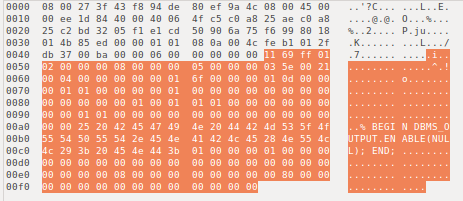
\includegraphics[width=0.9\textwidth]{tns-origin-sql.png}
\end{figure}

通过数字节,发现这个数据包也遵循前面的分析结果。所以此处的第 13 行 SQL 语句是经 sqlplus 转换后再发送给服务器的。

接下来的数据包发生了异变。如图 \ref{fig:tns-035e-header} 所示。

\begin{figure}[ht!]
    \caption{Oracle TNS 载荷数据包再次以 {\cf 0x035e} 开头}
    \label{fig:tns-035e-header}
    \centering
    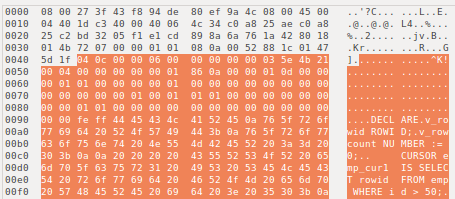
\includegraphics[width=0.9\textwidth]{tns-035e-header.png}
\end{figure}

至于载荷部分的数据再次以 {\cf 0x035e} 开头,我个人的理解是,不是所有的数据包都要以 {\cf 0x1169} 开头。
\footnote{前面提到的登陆后的第一条查询语句以 {\cf 0x035e} 开头是因为前面没有任何语句的需要处理,所以也就没有前面的 {\cf 0x1169} 数据包。}
前面已经提到过,{\cf 0x1169} 也是一种数据包,其操作意义是 {\ef Cursor Close All}。如果当前 SQL 语句的前一条语句没必要执行该操作,则下一条 SQL 语句前面不会夹带 {\cf 0x1169} 数据包,而是直接以 {\cf 0x035e} 开头。这种情况下,解析数据包的时候要做特别处理:

\begin{itemize}
    \item 如果数据包载荷以 {\cf 0x035e} 开头,则按照上面的偏移直接拿到 SQL 语句
    \item 如果载荷以 {\cf 0x1169} 开头,则简单记录一下数据包序列号之后,直接偏移到后面 {\cf 0x035e} 的地方,提取 SQL 语句。
\end{itemize}

对于上面的分析,可以再做一个实验。注意到,在 {\ff update.sql} 文件中,第 13 行的 SQL 语句 {\cf SET SERVEROUTPUT ON} 打开了服务器的一个选项,导致客户端每次都要发送一条如下的 SQL 语句到服务器

\begin{lstlisting}[language=sql]
BEGIN DBMS_OUTPUT.GET_LINES(:LINES, :NUMLINES); END;
\end{lstlisting}

包含这条语句的载荷数据包,其都是以 {\cf 0x035e} 开头的,不带 {\cf 0x1169} 数据包。而且在服务器端对该条数据包的返回载荷中,是以 {\cf 0x0b05} 开头的。如果将第 13 行去掉,则不会有这些信息,从而所有的数据包又再次携带 {\cf 0x1169} 数据包。

做这个实验的目的是为了说明某些 SQL 语句的执行会导致数据包载荷的头部发生一点变动,在解析的时候,需要注意一下。

\subsection{Oracle 12C TNS 协议的异同}\label{sec:12c-tns}
Oracle 12C 中的 TNS 协议与 11g 中又有不同,现将其异同列举一二:

\begin{itemize}
    \item 客户端登陆数据包中,第一条 connect 数据包格式是相同的,包括后面的 resend 数据包和 accept 数据包
    \item 表 \ref{tab:oracle-tns-data-type}、\ref{tab:tns-payload-data-type}、\ref{tab:oracle-tns-tti} 的意义基本保持不变

    \item 后面双方的 {\cf 0xdeadbeef} 数据包开始不同,数据包的整体长度放在第三、四个字节,载荷数据包类型放在了第 11 个字节(这个与 11g 中相同),所以在解析载荷类型时,要偏移 10 个字节
    \item {\cf 0x035exx} 之后偏移 73 个字节才到具体的 SQL 长度字节,而非 67 个字节
    \item 客户端发往服务器端的 {\cf 0x02} 类型的载荷数据包非常长,被分成三个数据包发送,而单个数据包的长度最大似乎为 1514 个字节。同样,服务器端返回的 {\cf 0x02} 数据包也很长,同样被分包。Oracle 11g 的情况是否如此,待定
\end{itemize}

更进一步的对比分析,后续再跟进。这样分析的目的是警告协议分析代码编写者,尽量分拆分析代码的逻辑,它们可能在不同的协议版本中都可以重用,只是组合方式的不同而已。

\subsection{Oracle 退出登陆数据包的组成}
[TODO]

\section{SQL Server 通信协议分析}

SQL Server 数据库中采用的的通信协议为 TDS\footnote{TDS 有多个版本,各个版本之间有些微差别,目前的大版本号为 {\ef 7},如果 SQL Server 版本大于等于 2005,则都支持 TDS {\ef 7} 了,所以优先支持 TDS {\ef 7}。},该协议的具体规格基本已经公开,而且有 FreeTDS 的开源实现,即通过 FreeTDS 即可模拟 客户端与 SQL Server 通信。

在 FreeTDS 中带有一个 {\cmdf tsql} 工具({\ff FreeTDS/src/apps/tsql}),用它即可模拟客户端行为:

\begin{lstlisting}
# tsql -S <sqlserver-ip> -U <username> -P <password>
\end{lstlisting}

此处服务器 IP 为 {\cf 192.168.37.129},用户名和密码按照服务器的安装配置来选择。

TDS 的协议流程基本上比较简单,就目前从 Wireshark 中抓取的数据包而言,其严格遵守基本的 ``一来一回'' 规则,在单次通信中(比如登录,输入查询语句等),基本就两个数据包就完成任务。不像 DRDA 那样,在单个操作中来回折腾多个数据包。

TDS 的数据包基本上格式如下

\begin{lstlisting}
    tcp_pkt
    |
    +-- type        : 2B
    +-- status      : 1B
    +-- length      : 2B
    +-- pkt_number  : 1B
    +-- window      : 1B
    +-- data        : nB
\end{lstlisting}

基本上前面 7 个字节为 TDS 数据包头,里面对一些基本信息进行了描述,便于后面对 {\cf data} 的解析。

对登录的数据包而言,其 {\cf data} 部分的格式如下:

\begin{lstlisting}
    data
    |
    +-- login_pkt_hdr   : 36B
    +-- len_and_offset  : 50B
    +-- client_name     : nB
    +-- username        : nB
    +-- password        : nB
    +-- app_name        : nB
    +-- server_name     : nB
    +-- lib_name        : nB
    +-- locale          : nB
\end{lstlisting}

{\cf data} 部分数据的特点是

\begin{itemize}
    \item {\cf data.login\_pkt\_hdr} 部分列出了很多关于数据包的属性信息,由于涉及字段较多,在此不详列
    \item {\cf data.len\_and\_offset} 则列出了自 {\cf data.client\_name} 到 {\cf data.locale} 各个字段在数据包中的偏移量以及长度
    \item 自 {\cf data.client\_name} 到 {\cf data.local},所有的数据均为 Unicode 编码,对于 ASCII 字符,其所占字节为 2,低字节补上 {\cf 0x00},例如,字符串 {\cf test} 的数据包格式为 {\cf 0x74 0x00 0x65 0x00 0x73 0x00 0x74 0x00}
\end{itemize}

对查询数据包而言,其 {\cf data} 部分的格式很简单,直接包含具体的查询语句,同理,其字符编码也为 Unicode 编码。

\section{IBM DB2 数据包协议分析}

DB2 数据库中采用的通信协议为 DRDA({\ef distributed rational database architecture}),其数据包结构为

\begin{lstlisting}
    tcp_pkt
    |
    +-- DRDA
    |   |
    |   + DDM
    |   |
    |   + parameter(optional)
    |   + ...
    |
    +-- DRDA
    |
    +-- ...

\end{lstlisting}

在单个 TCP 数据包中可能包含多个 {\cf DRDA} 数据包,在单个 DRDA 数据包中包含有一个 {\cf DDM}({\ef distributed database management}) 数据包和可选的一个或多个 {\cf parameter} 数据包。各个 {\cf DRDA} 包以及各个 {\cf parameter} 包之间均无任何分隔字符,{\cf DRDA}、{\cf DDM} 以及 {\cf parameter} 之间亦无分隔字符。

{\cf DDM} 数据包长度固定为 10 字节,其格式如下:

\begin{lstlisting}
    DDM
    |
    +-- length     : 2B
    +-- magic      : 1B
    +-- format     : 1B
    +-- correl_id  : 2B
    +-- length2    : 2B
    +-- code_point : 2B
\end{lstlisting}

其中

\begin{itemize}
    \item {\cf DDM.length} 指当前 DRDA 数据包总长度,包含一个 DDM 包长度以及若干 parameter 包长度
    \item {\cf DDM.magic} 基本上固定为 0xD0
    \item {\cf DDM.format} 包含一些属性信息,权作参考
    \item {\cf DDM.correl\_id} 目前不知道有什么用
    \item {\cf DDM.lenght2} 目前不知道有什么用
    \item {\cf DDM.code\_point} 指当前 DRDA 的数据包类型,根据该数据包类型可以知道这个 DRDA 是干什么用的
\end{itemize}

其中 {\cf DDM.format} 的位划分为:

\begin{lstlisting}
    format
    |
    +-- reserved         : 1b
    +-- chained          : 1b
    +-- continue         : 1b
    +-- same_correlation : 1b
    +-- dss_type         : 4b
\end{lstlisting}

{\cf DRDA.parameter} 的包格式为:

\begin{lstlisting}
    parameter
    |
    +-- length      : 2B
    +-- code_point  : 2B
    +-- data        : nB
\end{lstlisting}

其中 {\cf parameter.data} 在当前版本的协议中,如果用 DB2 自带的 {\cmdf db2} 程序与服务器通信,于原始数据的头尾分别会附加一个字节,可能是用于服务器端的识别,可以在解析时将其剪除。

这里面最重要的字段为两个 {\cf code\_point} 字段,分别为 {\cf DDM.code\_point} 以及 {\cf parameter.code\_point},它们分别代表具体的数据包类型,根据该类型,即可按照需求解析所需数据。

另外需要注意的一点是,在目前的分析情景中使用的是 DB2 自带的 {\cmdf db2} 工具作为客户端与 Windows 上安装的 DB2 服务器通信,在 Wireshark 中看到的是,对于标准 ASCII 字符,有些(并非全部,根据 {\cf parameter.code\_point} 而定) {\cf parameter.data} 的编码格式为 EBCDIC,而非通常的 ASCII 格式,比如,对于 ASCII 字符 {\cf 'd'}, EBCDIC 将其编码为 {\cf \verb|\204|},其十六进制为 {\cf 0x84}。如果需要解析这些数据,则需要将这些字节做相应的转换\footnote{关于转换映射,参见 \href{https://publib.boulder.ibm.com/infocenter/comphelp/v8v101/index.jsp?topic=\%2Fcom.ibm.xlf101a.doc\%2Fxlflr\%2Fasciit.htm}{这里}}。

\section{MySQL 数据包协议分析}
[TODO]

\section{超长 SQL 语句的处理}
为保持协议分析的正确性,分别对 SQL Server、MySQL 以及 Oracle 中超长 SQL 语句进行了测试,结果如下:

\begin{itemize}
    \item SQL Server 会对数据包进行分包,单个包的大小(包括协议头部字节)为 4Kb
    \item 使用 Linux 自带的 MySQL 客户端的测试结果为:MySQL 客户端对长度为 6Kb 的 SQL 语句没做任何处理,直接发送过去了,在服务器收到的是单个数据包,在 Wireshark 中看来是这样的。但是在底层的 TCP 协议上,还是对数据进行了分割,我检测到的分割长度为 4096 字节,即虽然 MySQL 协议(第七层)上不会对超长数据包做标识,但是第四层上对数据包还是有所处理。但这里不保证所有的情况都是这样子。
    \item 用 SQLPlus 测试时,Oracle 11g R2 直接忽略过长的 SQL 语句并报错:{\cf SP2-0027: Input is too long (> 2499 characters) - line ignored},据实测,SQL 语句的长度不能超过 2499(不含 2499,最长为 2498),此长度包括 SQL 语句后的 `{\cf ;}' 字符,但是如果换做其它客户端,可能该长度有所改变,即该长度是 sqlplus 工具的限制,因为当长度为 2499 时,Wireshark 根本没有抓到该数据包,即 sqlplus 没有将该长度的数据包发送出去,客户端本身就截留了该 SQL 语句。
\end{itemize}
